\chapter{Non-relational DBMS inside VO}

Typically, modern relational databases have shown little efficiency in certain applications using intensive data, like indexing of a large number of documents, sites rendering with high traffic, and streaming sites. Typical RDBMS implementations are tuned either for small but frequent reads and writes or a large set of transactions that have few write accesses. On the other hand NoSQL DB are optimized for read and append operations, and perform outstandingly where a relational DB would slow down. They are especially fast when large amounts of data have to be queried and if we consider that speed is more important than consistency. 

IVOA has a standard called Astronomical Data Query Language (ADQL) that users do not necessarily need to know, because he can pose a query with a GUI, as long as the query is translated into standard ADQL. The receiving service likewise converts the standard ADQL into whatever its own database servers need, but always inside relational model. For the reasons stated in chapter \ref{theproblem}, we propose the use of a different approach, the NoSQL technology.


\section{NoSQL}

A non-relational database just stores data without explicit and structured mechanisms to link data from different buckets to one another. 

NoSQL implementations used in the real world include 3TB Digg green markers (indicated to highlight the stories voted by others in the social network), the 6 TB of "ENSEMBLE" European Commission database used in comparing models and air quality, and the 50 TB of Facebook inbox search. 

NoSQL architectures often provide limited consistency, such as events or transactional consistency restricted to only data items. Some systems, however, provide all guarantees offered by ACID systems by adding an intermediate layer. There are two systems that have been deployed and provide for storage of snapshot isolation column: Google Percolator (based on BigTable system) and Hbase transactional system developed by the University of Waterloo. These systems use similar concepts in order to achieve distributed multiple rows ACID transactions with snapshot isolation guarantees for the underlying storage system in that column, wit no extra overhead in data management, no system deployment middleware or any maintenance introduced by middleware layer. 

Quite NoSQL systems employ a distributed architecture, maintaining data redundantly on multiple servers, often using distributed hash table. Thus, the system may actually escale adding more servers, and thus a server failure may be tolerated. 

There are different NoSQL DBs for different projects:

\begin{itemize}

\item Document oriented

  \begin{itemize}
    \item CouchDB
    \item MongoDB
    \item RavenDB
    \item IBM Lotus Domino
  \end{itemize}

\item Graph oriented

  \begin{itemize}
    \item Neo4j
    \item AllegroGraph
    \item InfiniteGraph
    \item Sones GraphDB
    \item HyperGraphDB
  \end{itemize}

\item Key-value oriented

  \begin{itemize}
    \item Cassandra
    \item BigTable
    \item Dynamo (Amazon)
    \item MongoDB
    \item Project Voldemort (LinkedIn)
  \end{itemize}

\item Multivalue

  \begin{itemize}
    \item OpenQM
  \end{itemize}  

\item Object Oriented
  
  \begin{itemize}
    \item Zope Object Database
    \item db4o
    \item GemStone S
    \item Objectivity/DB
  \end{itemize}

\item Tabular

  \begin{itemize}
    \item HBase
    \item BigTable
    \item LevelDB (BigTable open version)
    \item Hypertable
  \end{itemize}
  

\end{itemize}

They run on clusters of inexpensive machines.




\section{Advantages and uncertainties of NoSQL}

\begin{itemize}

\item \textbf{Elastic scaling}

DBA have relied on scale up — buying bigger servers as database load increases — rather than scale out — distributing the database across multiple hosts as load increases. However, as transaction rates and availability requirements increase, and as databases move into the cloud or onto virtualized environments, the economic advantages of scaling out on commodity hardware become irresistible.

Unlike RDBMS, the NoSQL databases are designed to expand transparently to scale and they are usually designed with low-cost in mind.


\item \textbf{Economics}

NoSQL databases typically use cheap clusters servers, while RDBMS tends to rely on expensive proprietary servers and storage systems. The result is a lower cost per transaction/second for NoSQL.


\item \textbf{Flexible data models}

Even minor changes to the data model of an RDBMS have to be carefully managed and may necessitate downtime or reduced service levels. NoSQL databases have a less strict (in the worst case) data model restrictions. NoSQL allows the application to store virtually any structure it wants in a data element. The result is that application changes and database schema changes do not have to be managed as one unit. In theory, this will allow applications to iterate faster.

\item \textbf{No need for DBAs}

RDBMS systems can be maintained only with the assistance of expensive and highly trained DBAs, while NoSQL databases are generally designed to require less management:  automatic repair, data distribution, and simpler data models lead to lower administration and tuning requirements and costs.



\end{itemize}


NoSQL systems have generated a lot of enthusiasm but there are still a lot of questions about its future:

\begin{itemize}

\item \textbf{Maturity}

RDBMS systems have been around for a long time. NoSQL evangelists will argue that their advancing age is a sign of their obsolescence, but mature RDBMS systems are stable. Most NoSQL alternatives are in pre-production versions with many key features yet to be implemented.

\item \textbf{Support}

Most NoSQL systems are open source projects, and although there are usually one or more firms offering support for each NoSQL database, these companies often are small start-ups.

\item \textbf{Expertise}

There are millions of developers with expertise using RDBMS. On ther other hand, NoSQL developers are, by far, a minority. This situation seems to change, but for now, it is easier to find experienced RDBMS programmers or DBA than NoSQL experts.

\end{itemize}

\section{MongoDB: a document oriented database}

MongoDB (from "humongous") is an open source document-oriented database system developed and supported by 10gen. It is part of the NoSQL family of database systems. Instead of storing data in tables as is done in a "classical" relational database, MongoDB stores structured data as JSON-like documents with dynamic schemas (MongoDB calls the format BSON), making the integration of data in certain types of applications easier and faster. 

As an example, we show some JSON code inserting a document in a Mongo DB:
\begin{lstlisting}
db.columns.insert( {
		table_name: "TAP_SCHEMA.schemas",
		column_name: "schema_name",
		utype: null,
		ucd: null,
		unit: null,
		description: "schema name for reference to TAP_SCHEMA.schemas",
		datatype: "VARCHAR",
		size: 64,
		principal: 1,
		indexed: 0,
		std: 0
	}
);
\end{lstlisting} 


10gen began Development of MongoDB in October 2007 and was not created to be just another database that tries to do everything for everyone. Instead, MongoDB was created to work with documents rather than rows, was extremely fast, massively scalable, and easy to use. In order to accomplish this, some features were excluded, namely support for transactions. 

%\begin{shaded}
A document database is more like a collection of documents. Each entry is a document, and each one can have its own structure. If you want to add a field to an entry, you can do so without affecting any other entry.
%\end{shaded} 



\subsection{Why MongoDB?}

A more detailed list of features is listed in \ref{features_mongo} , but as a summary, we have decided to use MongoDB for these reasons:

\begin{itemize}
\item It is open source code (available at \url{https://github.com/mongodb/mongo}).
\item Widely used in the NoSQL community.
\item It has full index support
\item Very easy to install and to connect through drivers with several programming languages like Java, Python, Ruby, C/C++, PHP or Scala.
\item It supports MapReduce paradigm.
\item It is possible to connect MongoDB with Hadoop (the \textit{de facto} big data processing and analytics platform \footnote{\url{http://hadoop.apache.org}}, allowing to to send MongoDB data into Hadoop MapReduce jobs, process the data and return it back to a MongoDB collection).
\end{itemize}

\subsection{Main features} \label{features_mongo}

\begin{itemize}

\item \textbf{Ad hoc queries} 
MongoDB supports search by field, range queries, regular expression searches. Queries can return specific fields of documents and also include user-defined JavaScript functions.

\item \textbf{Indexing} 
Any field in a MongoDB document can be indexed (indices in MongoDB are conceptually similar to those in RDBMS).

\item \textbf{Replication} 
MongoDB supports master-slave replication. A master can perform reads and writes. A slave copies data from the master and can only be used for reads or backup (not writes). The slaves have the ability to select a new master if the current one goes down.

\item \textbf{Load balancing} 
MongoDB scales horizontally using sharding (a shard is a master with one or more slaves). The developer chooses a shard key, which determines how the data in a collection will be distributed. The data is split into ranges (based on the shard key) and distributed across multiple shards. MongoDB can run over multiple servers, balancing the load and/or duplicating data to keep the system up and running in case of hardware failure. Automatic configuration is easy to deploy and new machines can be added to a running database.

\item \textbf{File storage} 
MongoDB could be used as a file system, taking advantage of load balancing and data replication features over multiple machines for storing files. This feature, GridFS, is included with MongoDB drivers and available for development languages. GridFS is used, for instance, in plugins for NGINX and lighttpd. In a multi-machine MongoDB system, files can be distributed and copied multiple times between machines transparently, thus effectively creating a load balanced and fault tolerant system.

\item \textbf{Aggregation} 
MapReduce can be used for batch processing of data and aggregation operations. The aggregation framework enables users to obtain the same results as the SQL GROUP BY clause.

Once we have seen the main features of MongoDB, we can move on to the language itself.
\end{itemize}


\subsection{The basics}

We must know four concepts to dig into MongoDB's world:

\begin{itemize}
\item Database: this concept is much like the RDBM counterpart.
\item Collection: we can see a collection and a table as the same thing.
\item Document: its equivalent in RDBM is the row, and a document is made up of fields.
\item Field: is a lot like a column.
\end{itemize}


\begin{table}
\begin{center}
\begin{tabular}{|l|l|}
\hline
\textbf{Relational} & \textbf{Document oriented} \\ 
\hline
Table & Collection\\
\hline
Row & Document\\
\hline
Column & Field \\
\hline
\end{tabular}
\end{center}
\caption{Differences between relational and NoSQL terms}
\end{table}



% \begin{figure}[H]
% \centering
% 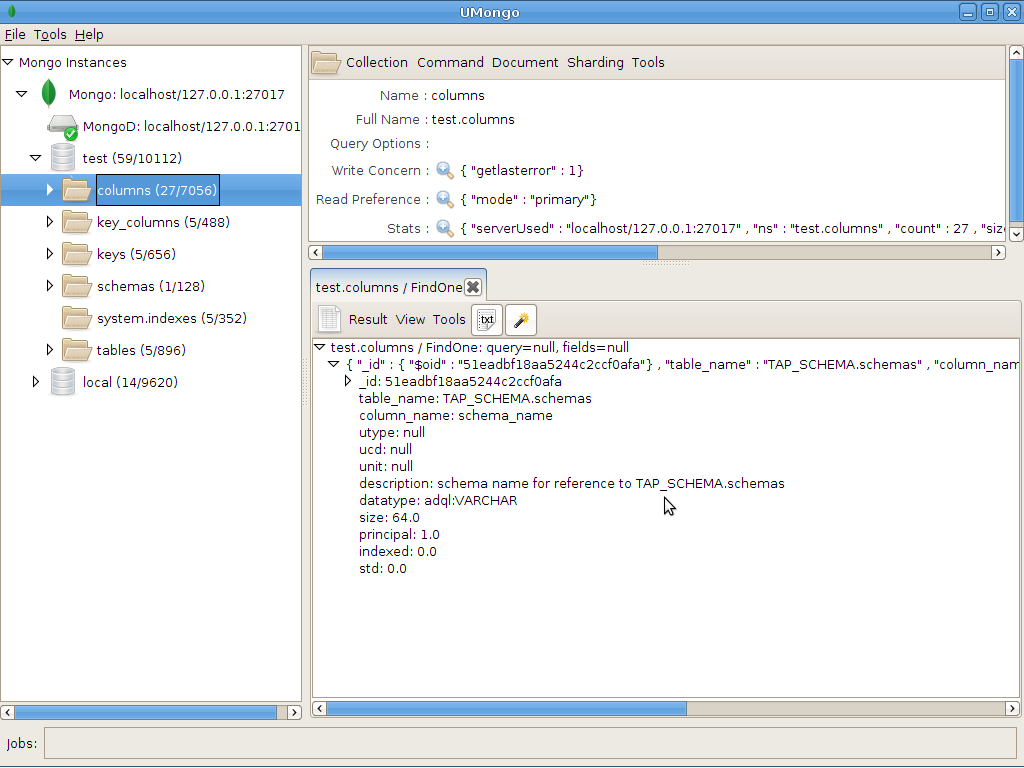
\includegraphics[width=11cm,height=8cm]{images/mongo_dia.png}
% \caption{Tree View for Tap Schema in MongoVue}
% \end{figure}


\subsubsection{SQL/Mongo syntax differences}

In this subsection we can see some differences in the DDL syntax used by both SQL and MongoDB. For the latter, we can call it from any language having a driver to connect to the DB or use the interactive shell (the code presented here uses this shell): 

\lstinputlisting[language=SQL]{src/sample01.sql}



\section{FITS alternative in MongoDB}

The first issue when working with FITS files is its inadequacy for storing information. In XXI century is difficult to maintain such storage model. So the first and more obvious solution would be replacing FITS headers with their counterparts in a non relational database. 

Another issue when working with FITS format is the great amount of possible key-value pairs in FITS headers. A possible solution for this problem could be use the features of MongoDB to translate FITS keywords into collections. So, we could create as much documents as needed, and storing them into MongoDB. Should we need to create supertypes of FITS headers, relations are also available in MongoDB through document linking (with no physical restriction in the sense of relational constraint). In this situation the schema flexibility means that we can model documents that share a similar structure but not enforced to have to same.

Another related problem is having multiple FITS formats \footnote{The IAU FITS Working Group (IAU-FWG) is the international control authority for the FITS (Flexible Image Transport System) data format: \url{http://fits.gsfc.nasa.gov/iaufwg/iaufwg.html}}, representing the users need for storing and handling the different information requirements:

\begin{itemize}
\item FITS Interferometry Data Interchange (FITS-IDI) Convention: conventions adopted for registering information from interferometric telescopes recordings. Used by the VLBA.
\item Single Dish FITS (SDFITS) Convention for Radio Astronomy Data: conventions used for the interchange of single dish data in radio astronomy. 
\item Multi-Beam FITS Raw Data Format Convention: conventions used at the IRAM 30m and APEX 12m mm/submm telescopes.
\item OIFITS: A Data Standard for Optical Interferometry Data: conventions used for exchanging calibrated, time-averaged data from astronomical optical interferometers.
\end{itemize}


We show now a logical layout using MongoDB features to solve the previously posed problem. Let's suppose we have several FITS files and we have to handle them as easy as possible.

For the sake of simplicity and clarity, we have not included all FITS keywords, focusing on the abstraction.

We can profit from MongoDB store units (collections, documents and fields). We could define as much kinds of documents as needed, sort of meta-documents, considering that there is no compulsory for them having the same structure. 

\paragraph{Solution}

Using just one collection and $n$ documents, one for each kind. If we are going to work with FITS-IDI, SDFITS, MBFITS and OIFITS, the code should be like this:

\begin{lstlisting}

db.fits_super.insert(
  convention: "FITS-IDI"
);

db.fits_super.insert(
  convention: "SDFITS"
);

db.fits_super.insert(
  convention: "MBFITS"
);

db.fits_super.insert(
  convention: "OIFITS"
);

\end{lstlisting}




Now, inserting the primary HDU for a  FITS-IDI header in MondoDB could not be easier. We start from a very simple FITS header like: 
\begin{verbatim}
SIMPLE = T 			/ Standard FITS format
BITPIX = 8 			/
NAXIS = 0 			/
EXTEND = T 			/
BLOCKED = T 			/
OBJECT = ’BINARYTB’ 		/
TELESCOP= ’VLBA ’ 		/
CORELAT = ’VLBA ’ 		/ added to header dump by EWG
FXCORVER= ’4.22 ’ 		/
OBSERVER= ’BL146 ’ 		/
ORIGIN = ’VLBA Correlator’ 	/
DATE-OBS= ’2007-08-23’ 		/
DATE-MAP= ’2007-08-31’ 		/ Correlation date
GROUPS = T 			/
GCOUNT = 0 			/
PCOUNT = 0 			/
END
\end{verbatim}

This code is very easy to translate into MongoDB syntax: 

\begin{lstlisting}

db.my_idi_collection.insert(
    supertype: "FITS-IDI", // it simulates a foreign key!
    SIMPLE: "T",
    BITPIX: 8,
    NAXIS: 0,
    EXTEND: "T",
    BLOCKED: "T",
    OBJECT: "BINARYTB",
    TELESCOP: "VLBA ",
    CORELAT: "VLBA ",
    FXCORVER: "4.22 ",
    OBSERVER: "BL146 ",
    ORIGIN: "VLBA Correlator",
    DATE-OBS: "2007-08-23",
    DATE-MAP: "2007-08-31",
    GROUPS: "T",
    GCOUNT: 0,
    PCOUNT: 0,
);

\end{lstlisting}

Now, we have our FITS header into a database with a document structure. We keep the same approach but in a very more usable and efficient way.



\section{MapReduce in MongoDB}

MapReduce, developed by Google, is a programming model and its implementation for processing (\textit{e.g.} raw data from telescopes) and producing (\textit{e. g.} representations of graph structure of systems) huge amounts of data. As the runtime controls the partitioning of the input data, controlling the program execution across several hundred or thousands of nodes and even controlling machine failures, the developers with low or none expertise at all in parallel programming can take advantage of this model with a very low learning curve.

MapReduce, usually, is used to solve problems involving big size datasets, up to several petabytes. For this reason, this model is used in distributed file systems, like HDFS \footnote{For a full specification of this filesystem, go to \url{http://hadoop.apache.org/docs/stable/hdfs_design.html}}.

The MapReduce model allows to write a map function which takes a key/value pair, operates on it (performs object detection) and returns a new set of key/value pairs (source list). The reduce function then aggregates/merges all the intermediate data (builds an object catalog on a stacked source list). Many problems in astronomy naturally fall into this model because of the inherent parallelizability of many astronomical tasks.

\begin{figure}[H]
\centering
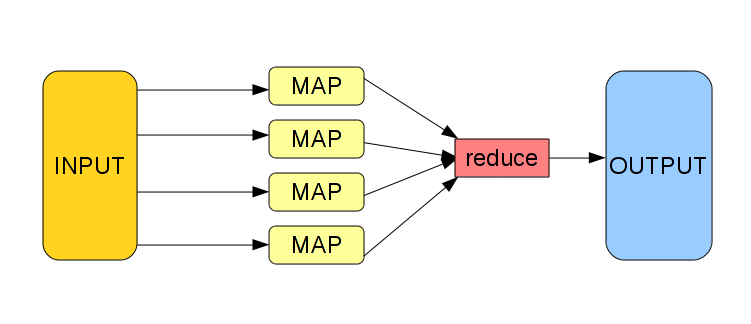
\includegraphics[height=8cm]{images/map_reduce_chart.png}
\caption{MapReduce concept}
\end{figure}

To finish this chapter, we have developed a simple MapReduce job to show its use inside the context we are working on.

\lstinputlisting[language=Java]{src/map_reduce_01.js}


\section{Rewriting ALMA Science Archive}

\begin{figure}
\centering
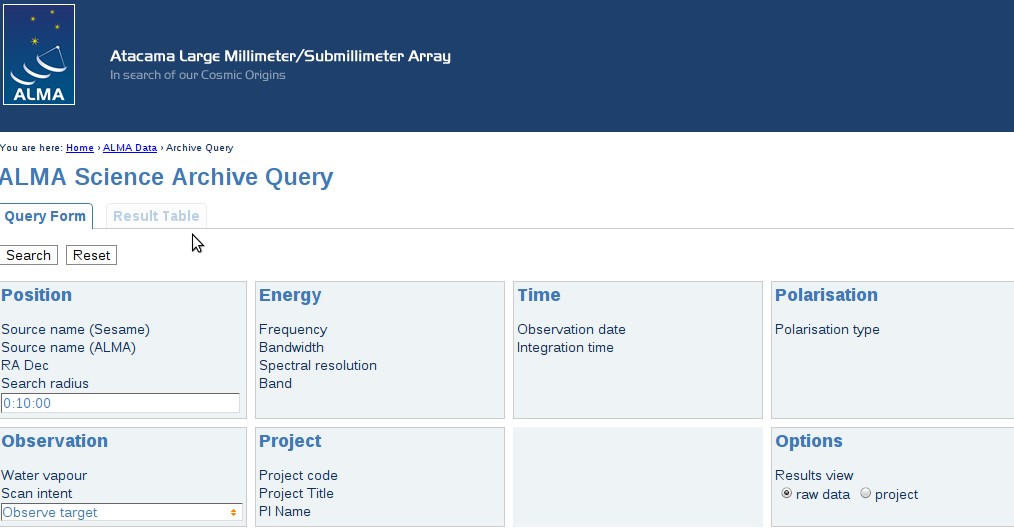
\includegraphics[height=8cm]{images/aq.png}
\caption{ALMA Science Archive Query}
\end{figure}


ALMA Science Archive (ASA) is the interface for querying ALMA data. Despite all ALMA information can be accessed from the Archive, ASA provide a optimized way to access the data in a scientific way. One of the requirements of ASA design was to provide a search and query tool which allows several parameters (position, frequency, telescope related parameters, etc.). It has two major components: the DB, which is a plain relational database with denormalized structure and the interface, built as a web application.

%\begin{figure}
%\centering
%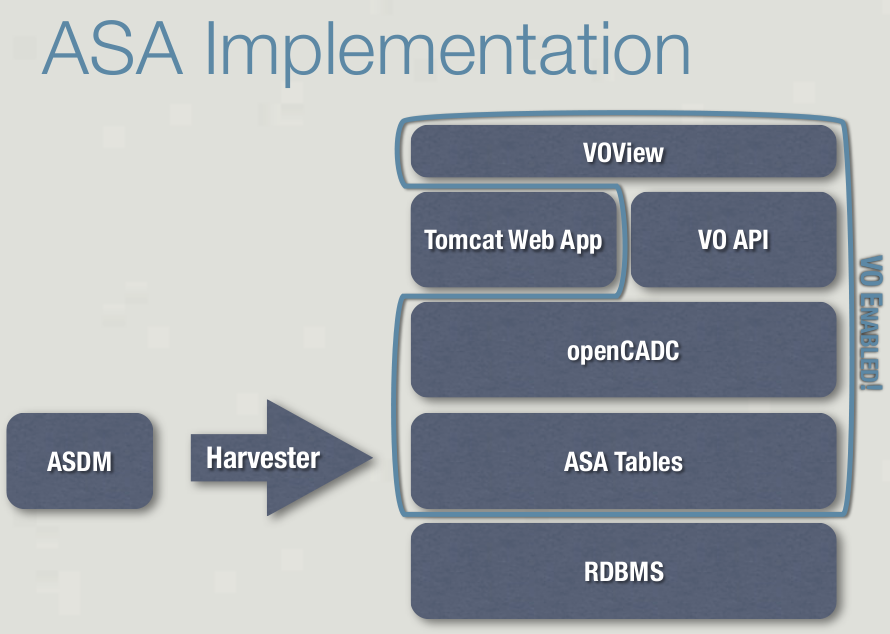
\includegraphics[width=14cm,height=8cm]{images/asa_implementation.png}
%\caption{ALMA implementation, from  %\href{http://amiga.iaa.es/FCKeditor/UserFiles/File/VOandALMAarchive_web.pdf}{AMIGA-IAA Group Web}}
%\end{figure}


The VO Technologies used in the ALMA Archive are (discussed in \ref{vochapter}):

\begin{enumerate}
\item VO Data Models
\item Software
  \begin{enumerate}
    \item OpenCADC
    \item VOView: a utility for viewing large data tables within a Web browser, reformatting a table in XML into HTML requested by the browser.
  \end{enumerate}
\end{enumerate}

\subsubsection{Java and MongoDB in ASA}

Let's see some simple examples from ALMA query interface: 

\newpage
\begin{lstlisting}
/* code from TapSchemaDAO.java */

// SQL to select all rows from TAP_SCHEMA.colums.
private static final String SELECT_COLUMNS_TEMPLATE = 
  "select table_name, column_name, description, utype, ucd, unit, datatype, type_size " +
  "from %s.asa_columns ";

// List of TAP_SCHEMA.columns
List<ColumnDesc> columnDescs = jdbc.query(
  String.format(SELECT_COLUMNS_TEMPLATE, schemaName),
  new ColumnMapper()
);


\end{lstlisting}

% Now, we dive into a yet simple example, whose original version, coded in Java for a RDMS can be found online \footnote{\url{https://github.com/jantoniomagro/Misc/blob/master/TapSchemaDAO.java}}. We show here just the relevant code to see the Mongo version in Java.
% 
% \lstinputlisting[language=SQL]{/home/jose/Escritorio/TFM/src/TapSchemaDAO.java}